\documentclass{article}

\usepackage{fullpage}
\usepackage{multicol}
\usepackage{amsmath}
\usepackage{bm}

\renewcommand{\vec}[1]{\underline{\textbf{#1}}}
\newcommand{\veci}{\bm{\hat{\imath}}}
\newcommand{\vecj}{\bm{\hat{\jmath}}}
\newcommand{\veck}{\bm{\hat{k}}}
\newcommand{\e}{\varepsilon}
\newcommand{\de}{\delta}
\newcommand{\kd}{\delta_{i, j}}
\newcommand{\at}{\e_{i, j, k}}

\usepackage{tikz}
\usetikzlibrary{shapes.geometric, positioning}

\usepackage{float}


\newtheorem{example}{Example}
\newtheorem{solution}{Solution}

\title{Suffix Notation}
\author{James Arthur}

\begin{document}
\maketitle
\tableofcontents\newpage


\multicols{2}
[\section{Lecture 1: Basic Definitions}]

\subsection{Suffix Notation}

Let there be a vector $\vec{c} = \vec{a} + \vec{b}$, where $\vec{a} = a_1 \veci + a_2 \vecj + a_3 \veck$ and $\vec{b} = {b}_1 \veci + {b}_2 \vecj + {b}_3 \veck$. Then $\vec{c} $ is equivalent to:

$$ c_i = a_i + b_i $$

In suffix notation:
$$ c_j = a_j + b_j \qquad j = 1, 2, 3 $$

The inner product of two vectors:
\begin{align*}
   a\cdot b &= a_1b_1 + a_2b_2 + a_3b_3\\
   &= \sum_{j=1}^3{a_jb_j}
\end{align*}
For a vector $\vec{a} = a_i$, $i$ is a free index. For the dot product above: $\displaystyle{\sum_{j=1}^3{a_jb_j}} $, $j $ is a dummy suffix.

For suffix notation, an index cannot be repeated more than two times in an equation.
\fbox{\parbox{0.475\textwidth}{
\begin{example}
  Write $(a\cdot b)(c \cdot d) $ in suffix notation
\end{example}
\begin{solution}
Here we take that: $$a\cdot b = a_jb_j \quad j = 1, 2, 3 $$ and that $$c\cdot d = c_id_i \quad i = 1, 2, 3 $$ Now we can say that $$(a\cdot b)(c \cdot d) = a_jb_jc_id_i \quad i,j=1,2,3$$
\end{solution}
}}\vspace{10pt}
\fbox{\parbox{0.475\textwidth}{
\begin{example}
  Write $a_jb_ic_j $ in normal vector notation
\end{example}
\begin{solution}
We know that $$ a_jb_ic_j = a_jc_jb_i $$ Which is: $$ (a \cdot c) b $$
\end{solution}
}}\vspace{10pt}
\fbox{\parbox{0.475\textwidth}{
\begin{example}
  Write the vector notation $\vec u + (\vec{a}\cdot \vec{b})\vec v = |\vec a|^2(\vec b \cdot v)\vec a $ in suffix notation
\end{example}
\begin{solution}
We know that $$ a_jb_ic_j = a_jc_jb_i $$ Which is: $$ (a \cdot c) b $$
\end{solution}
}}\vspace{10pt}
\fbox{\parbox{0.475\textwidth}{
\begin{example}
  Write the vector notation $\vec u + (\vec{a}\cdot \vec{b})\vec v = |\vec a|^2(\vec b \cdot v)\vec a $ in suffix notation
\end{example}
\begin{solution}
  Firstly:
  $$ \left[\vec u + (\vec{a}\cdot \vec{b})\vec v\right]_i = \left[|\vec a|^2(\vec b \cdot v)\vec a\right]_i$$ Then,
  $$u_i + (a_jb_j)v_i = a_ja_jb_lv_la_i \qquad j,l = 1, 2, 3$$
\end{solution}
}}\vspace{10pt}


\subsection{The Kronecker Delta $\kd $}

The function is defined:

$$ \kd = \begin{cases}
1, & i = j\\
0, & i \neq j\\
\end{cases} $$

The suffixes $ i$ and $j$ can each take the values $1, 2, 3$ so $\kd$ has nine elements.

We can write the function as the identity matrix:

$$ \kd = \begin{pmatrix}
1 & 0 & 0 \\
0 & 1 & 0 \\
0 & 0 & 1 \\
\end{pmatrix}
$$

$ \kd$ is called a substitution tensor, since it's effect when multiplied by $a_j$ is to replace $j$ with $i$.
\begin{align*}
\kd a_j &= \sum_{j=1}^3 {\kd a_j}\\
&= \delta_{i1}a_1 + \delta_{i2}a_2 + \delta_{i3}a_3 \\
&= \delta_{11}a_1 + \delta_{12}a_2 + \delta_{13}a_3 \\
&\quad+ \delta_{21}a_1 + \delta_{22}a_2 + \delta_{23}a_3\\
&\quad+ \delta_{31}a_1 + \delta_{32}a_2 + \delta_{33}a_3\\
&= a_1 + a_2 + a_3
\end{align*}

From this we can say: $\kd a_i =  a_j$ and $\kd a_j = a_i$\vspace{10pt}

\fbox{\parbox{0.425\textwidth}{ \begin{example} $\kd $ and dot product  \end{example} \begin{solution} \begin{align*}
  a\cdot b &= a_ib_i \quad i=1,2,3\\
  &= \kd a_jb_i \\
  &= a_j\kd b_i\\
  &= a_jb_j\\
\end{align*} \end{solution} }}\vspace{10pt}


\subsection{The Alternating Tensor, $\e_{i, j, k}$ }

$ \at$ is useful for manipulating expressions involving the cross product of two vectors and curl of a vector.

$\at = \begin{cases}
  +1 & \text{ if } (i, j, k) = (1, 2, 3),\, (2, 3, 1) \text{ or } (3, 1, 2)\\
  -1 & \text{ if } (i, j, k) = (3, 2, 1),\, (2, 1, 3) \text{ or } (1, 3, 2)\\
  0 & \text{if any of } i, j, k \text{ are equal} \\
\end{cases}$
\begin{figure}[H]
  \centering
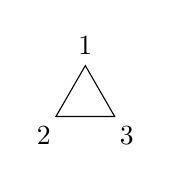
\begin{tikzpicture}[baseline=(a.south)]
   \node[
     draw,
     regular polygon,
     regular polygon sides=3,
     text width=.2em
     ] (a) {};
      \node[above=0pt of a] {$1$};
      \node[below=0pt of a] {$2 \qquad\,\,\, 3$};
 \end{tikzpicture}
\end{figure}
The $+1$ case can be also written as 1, 2 or 3 are in clockwise order. So if you take a triangle and then go clockwise around it from the first element, that the order they are in. The $-1$ are in anticlockwise order. Hence meaning the opposite of clockwise.\\

The six non-zero elements of $\e_{ijk}$:
\begin{align*}
  &\e_{123} = \e_{231} = \e_{312} = +1\\
  &\e_{321} = \e_{213} = \e_{132} = -1 \\
  &\e_{ijk} = 0, \text{ otherwise} \\
\end{align*}

We can take that; $\e_{ijk} = \e_{jki} $ as they are in clockwise order. This also imples $\e_{ijk} = - \e_{jik}$ because if $ijk $ are in clockwise order then $jik$ must be in counterclockwise order.

\subsection{$\e_{i, j, k}$ and cross product}

Let $\vec a = {a}_1 \veci + {a}_2 \vecj + {a}_3 \veck$ and $\vec b = {b}_1 \veci + {b}_2 \vecj + {b}_3 \veck$. Then their cross product is:
$$ \vec a \times \vec b = \left|\begin{matrix}
  \veci & \vecj & \veck \\
  a_1 & a_2 & a_3 \\
  b_1 & b_2 & b_3 \\
\end{matrix}\right| $$

and in suffix notation, we can write the above as; $(\vec a \times \vec b)_i = \e_{ijk} \, a_jb_k $ where $j, k$ are dummy suffixes and must be summed over $1$ to $3$.

\subsection{$\e_{ijk}$ and the scalar triple product}

We can take the scalar triple product, $\vec a \cdot \vec b \times \vec c$, then we can do the following:

\begin{align*}
  \vec a \cdot \vec b \times \vec c &= a_i (\vec b \times \vec c)_i\\
  &= a_i \e_{ijk} b_j c_k \\
  &= \e_{ijk} a_i b_j c_k \\
  &= c_k \e_{ijk} a_i b_j \\
\end{align*}

from the above we show that $\vec a \cdot \vec b \times \vec c = \vec c \cdot \vec a \times \vec b $. We can expand $\e_{ijk}\, a_i\, b_j\, c_k$ to get:
\begin{align*}
  &= \e_{123}a_1b_2c_3 + \e_{231}a_2b_3c_1 + \e_{312}a_3b_1c_2 \\
  &\quad+ \e_{321}a_3b_2c_1 + \e_{213}a_2b_1c_3 + \e_{132}a_1b_3c_2 \\
  &= a_1b_2c_3 + a_2b_3c_1 + a_3b_1c_2 - a_3b_2c_1 - a_2b_1c_3 - a_1b_3c_2
\end{align*}

which is the expanded form of the triple scalar product.

\subsection{A relation between $\e_{ijk}$ and $\kd$}
We are going to prove the following statement:
$$ \e_{ijk}\e_{klm} = \delta_{il}\delta_{jm} - \delta_{im}\delta_{jl} $$
Since all of the coordinate axis are the same, just consider $\displaystyle{i = 1}$:\\

\noindent
If then $\displaystyle{j = 1}$, we get that $\displaystyle{\e_{11k} = 0}$ and so LHS $\displaystyle{= 0}$. Then considering the RHS, we get that $\displaystyle{\delta_{1l}\delta_{1m} - \delta_{1m}\delta_{1l} = 0}$, so equation holds.\\

\noindent
If $\displaystyle{j=2}$, then $\displaystyle{\e_{ijk} = {\e_{12k} = 0}$, unless $\displaystyle{k=3}$, so then only $\displaystyle{k=3}$ contributes to the sum. So $\displaystyle{\e_{klm} = \e_{3lm}}$, so zero unless $l$ and $m$ are $1$ and $2$. So we can conclude that $\displaystyle{\e_{ijk}\e_{klm} = \e_{123}\e_{312}}$ or $\e_{123}\e_{321}$, so the LHS is either $\pm 1$. Looking at RHS, we have either: $\delta_{11}\delta_{22} - \delta_{12}\delta_{21}$ or $\delta_{12}\delta_{21} - \delta_{11}\delta_{22}$. This gives $\pm 1$ in the same perumtation as the LHS. So equation holds.

\noindent
If $\displaystyle{j = 3}$, then 














\end{document}
